\chapter{Gekoppelte Pendel}
Gekoppelte Pendel sind solche Pendel, zwischen denen ein Energieaustausch stattfindet. Die dadurch ausgeführten Schwingungen werden auch Koppelschwingung genannt. In jedem Pendel wirkt ein Richtmoment, das durch die Schwerkraft hervorgerufen wird und bestrebt ist, das Pendel in die Ruhelage zurückzuziehen. Außerdem macht sich die vorhandene Kopplung in Form eines zusätzlichen Richtmoments bemerkbar, das so wirkt, dass die Feder möglichst entspannt wird.
Häufig versteht man unter gekoppelten Pendeln zunächst die Wechselwirkung zwischen zwei Pendeln. Das Konzept lässt sich jedoch auf beliebig viele Pendel anwenden. Mehrere gleiche Pendel, die in einer Reihe angeordnet mit ihren unmittelbaren Nachbarn wechselwirken, bezeichnet man als Schwingerkette.
\\
Das Richtmoment D ist bei einer mechanischen Torsion die Proportionalitätskonstante zwischen dem anliegenden Drehmoment
M und dem Drehwinkel $\phi$ :
\begin{center}
$\vec{M}= D\vec{\phi}$\\
\end{center}
Die Kreisfrequenzen der harmonischen Pendelbewegungen:
\begin{center}
 $\omega_{gl} = \sqrt{\dfrac{g}{L}}$ \\
 $\omega_{geg} =\sqrt{\dfrac{g+2k}{L}}$
\end{center}
Schwebungsdauer $T_{s}$ :
\begin{center}
 $T_{s}= 2\cdot\dfrac{T_{gl}\cdot T_{geg}}
{T_{gl}-T_{geg}}$
\end{center}
Der Kopplungsgrad K ist ein Maß für die Stärke der Kopplung und ist gegeben durch:
\begin{center}
 $K= \dfrac{Dr^2}
 {D+Dr^2}$
\end{center}
\begin{minipage}{\textwidth}
 \centering
 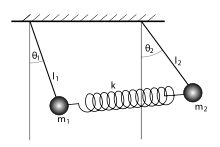
\includegraphics[width=0.7\textwidth]{gekpendel}
 \captionof{figure}{Gekoppelte Pendel}
 \label{fig:Abb4}
\end{minipage}
\section{Fragen zur Vorbereitung}
1. Ist die Eigenkreisfrequenz
$\omega_{geg}$ bei gegenphasiger Schwingung kleiner, gleich oder größer als bei gleichsinniger Schwingung  $\omega_{gl}$?\\
Bei gleichsinniger Schwingung ändert sich die Länge der Feder und somit ihre Spannung nicht. Somit werden keine zusätzlichen Drehmomente auf die Pendel ausgeübt. Sie schwingen dann unabhängig voneinander: $ \omega_{gl}=\omega_{0}$ (Diese Frequenz würde sich auch ohne Kopplungsfeder einstellen.) \\
Bei gegensinniger Schwingung wird die Feder periodisch verformt und übt zusätzliche zeitlich veränderliche Drehmomente auf die Pendel aus. Je weiter z.B. beide Pendel nach außen schwingen, desto stärker werden sie von der Feder zurückgezogen, Es ergibt sich eine symmetrische Schwingung der beiden Pendel, deren Eigenkreisfrequenz  $\omega_{geg}$ durch die zusätzlichen Drehmomente allerdings größer ist als $\omega_{0}$\\
\\2. Welche Bedeutung haben gekoppelte Schwingungen in der Molekülphysik?\\
In Molekülen kommt es zu unterschiedlich starken Bindungen  zwischen den einzelnen beteiligten Atomen. Diese kann man sich als unterschiedlich starke Federn vorstellen. Also schwingt dann bei Anregung nicht nur ein Atom oder eine isolierte Bindung, sondern durch Kopplung der Bindungen auch die umliegenden Bindungen bzw. Atome.\\
\\3. Wie kann man Schwebungen zum Stimmen von Musikinstrumenten verwenden? Warum eignet sich diese Methode insbesonders bei tiefen Frequenzen?\\
Das Instrument wird solange auf den Kammerton als Referenzton eingestimmt, bis keine Schwebung mehr zu hören ist. Bei Schwebung treten Lautstärkeschwankungen auf. Bei hohen Frequenz sind sie zu schnell aufeinander folgend und somit schwerer zu erkennen. Deswegen eignet sich diese Methode besonders bei tiefen Frequenzen.\\
\\4. Wie kann man mit Schwebungen sehr hohe Frequenzen messen?\\
Voraussetzung ist, eine Schwingung gleicher Amplitude und ähnlicher Frequenz erzeugen zu können. Überlagert man die zu messende Schwingung mit der Referenzschwingung, so entsteht eine Schwebung, deren Schwebungsfrequenz sich weit unter der zu messenden Frequenz befindet und somit einfach zu bestimmen ist. Mit Hilfe der nun vorhandenen Schwebugsfrequenz und der Referenzfrequenz kann die noch unbekannte Frequenz erschlossen werden.\\
\\5. Wie kann mittels eines sog. FRAHMschen Schlingertanks die Schlingerbewegung eines großen Schiffs verringert werden (Schiffs-Stabilisator)?\\Ein Schlingertank ist ein mit Wasser gefüllter Tank im Rumpf eines Schiffes, der Schwankungen um die Längsachse (das sogenannte Rollen) dämpfen soll.\\
Der von Frahm im Jahr 1910 patentierte Flüssigkeitsdämpfer besteht aus einem Uförmigen Rohrsystem gefüllt mit  z.B. Wasser. Der Flüssigkeitsdämpfer diente ursprünglich zur Dämpfung der Rollbewegung von Schiffen und gilt als einer der ersten Schwingungsdämpfer. Durch die Strömung der Flüssigkeitssäule wird die gleiche dämpfende Wirkung wie bei den mechanischen Schwingungsdämpfern verursacht. Die Eigenfrequenz sowie das Dämpfungsverhalten des Flüssigkeitsdämpfers werden über die Geometrie des Rohrsystems bestimmt. \\
Im Wesentlichen ist es ein Wasserpendel, das auf die Eigenresonanz des Schiffes abgestimmt ist. Treffen seitlich Wellen auf das Schiff, sind im Resonanzfall die Phase der Schiffsschwingung und die der stoßenden Wellen um $\pi/2$ verschoben. Nun bewegt sich das Wasser im Tanksystem (Zwei miteinander verbundene Tanks an den Seiten des Schiffs).  Stimmt die Eigenfrequenz des Wasserpendels mit dem des Schiffs überein, ergibt sich noch eine weitere Phasenverschiebung um $\pi/2$ . Letztendlich addieren sich die beiden Phasenverschiebung zu $\pi=180 $ Grad, sodass die gegenphasige Bewegung die Schlingerbewegeung des Schiffes dämpft.
\section{Durchführung}
Bauen Sie ein gekoppeltes Pendel auf. Achten Sie insbesonders auf die
Nadellager der beiden Pendel: die Nadeln sind sehr spitz, daher empfindlich; darüber hinaus könnten
Sie sich bei unsachgemäßem Umgang an den Spitzen verletzen.
Die Kopplungsfeder wird vorerst noch nicht verwendet.
Verbinden Sie die Winkelsensoren mit dem Messverstärker (Verstärkungsfaktor 10). Schließen Sie
den Ausgang des Messverstärkers an das Oszilloskop und an das USB-Multimeter an. Über das USB
Multimeter können Sie die Daten mit einer Auflösung von 2 Hz in eine Datei schreiben. Die Daten
werden anschließend über die Datenvisualisierung qtiplot ausgewertet.
Achtung: der Dezimalpunkt des Datensatzes muss ggfs. in ein Dezimalkomma ersetzt werden,
damit es von qtiplot richtig interpretiert werden kann!
\begin{itemize}
 \item 1. Justieren Sie bei absolutem Stillstand der Pendel den Offset der Winkelsensoren auf 0,0V.
 \item 2. Lenken Sie nun eines der Pendel leicht aus und beobachten Sie die Schwingung. Nehmen Sie über die Winkelsensoren und den Messverstärker einen Datensatz auf. Bestimmen Sie die Schwingungsdauer $T_{01} =\dfrac{2 \pi }{\omega_{01}}$. Wiederholen Sie den Messvorgang für das zweite Pendel und stellen Sie sicher, dass im Rahmen der Messgenauigkeit $T_{01}= T_{02} $ gilt.
 \item3. Verbinden Sie nun die Pendel über die Kopplungsfeder miteinander. Notieren Sie sich die Position der Befestigungsstelle.
 \item4. Zeichnen Sie die Schwingung auf, wenn beide Pendel in Phase sind und bestimmen Sie daraus die Periodendauer $T_{gl}$.
 \item5. Zeichnen Sie die Schwingung auf, wenn beide Pendel gegenphasig sind und bestimmen Sie daraus die Periodendauer $T_{geg}.$
 \item6. Lenken Sie nun ein Pendel aus der Ruhelage aus und erzeugen so gekoppelte Schwingungen.
 Zeichen Sie die gekoppelten Schwingungen auf und bestimmen Sie daraus die Oszillationsperiode Tm und die Schwebungsdauer $T_S.$
 \item7. Vergleichen Sie die erhaltenen Werte mit denen, die Sie für die natürlichen Perioden $T_{gl}$ und $T_{geg}$ zuvor berechnet haben. Berücksichtigen Sie eine kurze Fehlerbetrachtung.
 \item 8. Bestimmen Sie den Kopplungsgrad, indem Sie ein Pendel um eine bestimmte Strecke aus der
 Ruhelage auslenken und die Auslenkung des anderen Pendels messen. Wiederholen Sie die
 Messung für mindestens drei unterschiedliche Auslenkungen, sofern Sie noch über ausreichend
 Zeit verfügen.
 \item 9. Wiederholen Sie Aufgabe 8 bis 6 für einen andern Kopplungsgrad, indem Sie die Feder an
 einem anderen Punkt der Pedelstange befestigen.
\end{itemize}